\documentclass[fontsize=11pt]{article}
\usepackage{amsmath}
\usepackage[utf8]{inputenc}
\usepackage[margin= 0.75in]{geometry}
\usepackage{graphicx}
\graphicspath{ {./Images/} }

\title{CSC110 Project Proposal: \#ClimateChange}
\author{Faizah Sayyid, Tina Zhang, Courtney Amm, Poorvi Sharma}
\date{Friday, November 6, 2020}

\begin{document}
\maketitle

%=============================================================
% Problem Description and Research Question
%=============================================================

\section*{Problem Description and Research Question}

\qquad For our project we wish to analyze public perspectives and general engagement on the topic of climate change by examining tweets. More specifically, we want to find out which climate change related topics and events gain popularity on twitter, and which are left out of the conversation. Of course, Twitter users are not representative of the general population, since only a small percentage of people use twitter, and since twitter users tend to follow and interact with users who are similar to them. In addition, popular opinions on twitter are often influenced by overactive twitter users. However, twitter can still show us how the public behaves and reacts to climate change, and how they can influence the media and government to act on and generate awareness about climate change. Thus, we will analyze a large set of tweets from over years and assess whether people are talking about climate change related events, and how people at the global level feel about climate change. 

\vspace{0.5 cm}

Starting meaningful and informative conversations about climate change is an important way of raising awareness about this relevant and pending world issue. In the modern age, our awareness of different views and ongoing conversations in the world is in large part due to social media platforms such as Twitter. As such, Twitter may actually be able to give us insight into how the public views and engages in topics related to climate change. Furthermore, Twitter is a platform where many environmental activists organize protests, share information and resources about climate change related events and natural disasters, and attempt to convince people in power to make changes in order to decrease the threat of climate change. On the other hand, it is also a platform where users can spread misinformation and make false claims such as “climate change is a hoax”. As climate change becomes an increasing threat, it is important to understand how the global population stands on this issue, and whether enough people are talking about it.

\vspace{0.5 cm}

Therefore, the question we want to explore for this project is: \textbf{what can twitter tell us about public conversations on climate change at the global scale?}

%=============================================================
% Dataset Description
%=============================================================

\section*{Dataset Description}

The following datasets are the ones we might use:
\begin{enumerate}
\item\textbf{Harvard Dataverse: GWU Libraries Dataverse: Climate Change Tweets Ids (text):} 
\\This dataset contains tweet ids of 39,622,026 tweets related to climate change. They were collected using the POST statuses/filter method of the Twitter Stream API using Social Feed Manager. They used the track parameter with the following keywords: \#climatechange, \#climatechangeisreal, \#actonclimate, \#globalwarming, \#climatechangehoax, \#climatedeniers, \#climatechangeisfalse, \#globalwarminghoax, \#climatechangenotreal, climate change, global warming, climate hoax

\item\textbf{Kaggle: Twitter Climate Change Sentiment Dataset (csv):} This dataset aggregates tweets pertaining to climate change collected between Apr 27, 2015 and Feb 21, 2018. In total, 43943 tweets were annotated. Each tweet is labelled independently by 3 reviewers. This dataset only contains tweets that all 3 reviewers agreed on (the rest were discarded). Each tweet is labelled as one of the following classes:
    \begin{itemize}
        \item2(News): the tweet links to factual news about climate change
        \item1(Pro): the tweet supports the belief of man-made climate change
        \item0(Neutral): the tweet neither supports nor refutes the belief of man-made climate change
        \item(Anti): the tweet does not believe in man-made climate change
    \end{itemize}
The distribution of the data:

\begin{center}
    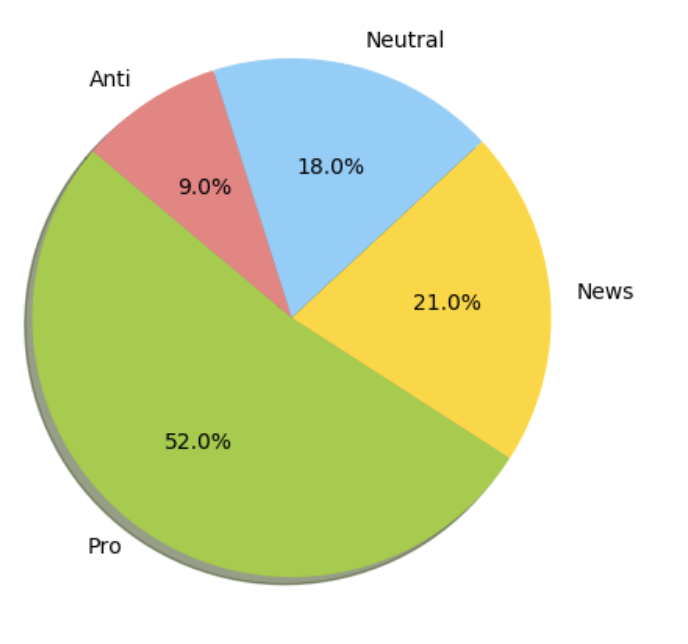
\includegraphics[width=8.5cm, height=8cm]{Images/Kaggle_Pi_Chart.png}
\end{center}

\item\textbf{Data.world: Sentiment of Climate Change (csv):} Contributors evaluated tweets for belief in the existence of global warming or climate change. The possible answers were "Yes" if the tweet suggests global warming is occurring, "No" if the tweet suggests global warming is not occurring, and "I can't tell" if the tweet is ambiguous or unrelated to global warming. They also provide a confidence score for the classification of each tweet.
\end{enumerate}
We may also use these to create our own datasets or use the data to do computations:
\\\textbf{Carbon Brief} has mapped every extreme-weather attribution study published to date. The map shows 355 extreme weather events and trends across the globe for which scientists have carried out attribution studies. The different symbols show the type of extreme weather; for example, a heatwave, flood or drought. The colours indicate whether the attribution study found a link to human-caused climate change (red), no link (blue) or was inconclusive (grey).

\begin{center}
    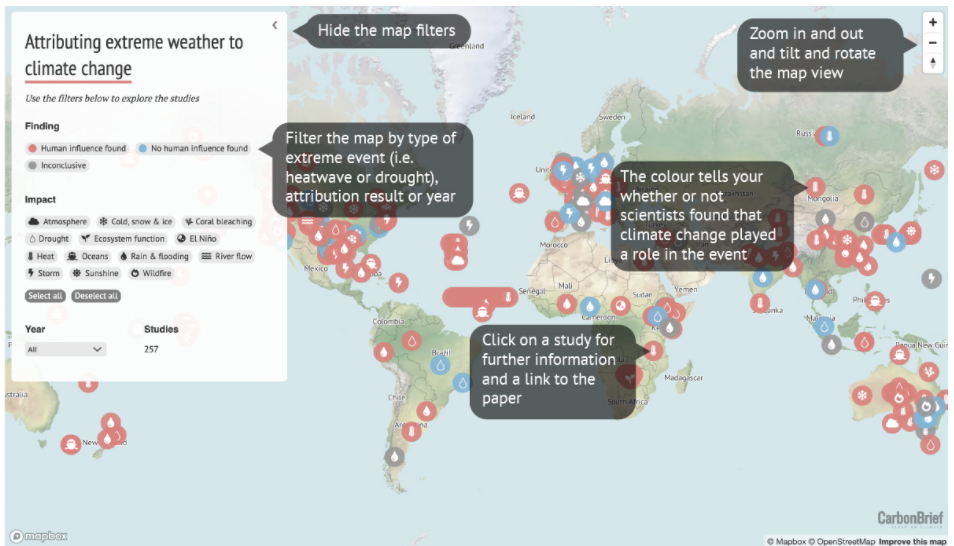
\includegraphics[width=10cm, height=6cm]{Images/Climate_Data_Map.png}
\end{center}

%=============================================================
% Computational Plan
%=============================================================

\section*{Computational Plan}

\qquad We plan on filtering the twitter data set by geographical locations, dates, as well as hashtags and keywords. The filtered data will be grouped into countries, sorted by time, and aggregated by keywords as a mapping. We will also use plotly to display the data. If time allows it, we also plan on applying sentiment analysis to the context of these tweets to determine the user’s perspective on the issue. 

\vspace{0.5 cm}

The final product of our project will be a twitter map displayed visually and interactively using plotly. Users will be able to input a certain climate related hashtag or keyword to see the popularity of this topic in the world in colors, and possibly even the perspectives of these countries on this topic. There will also be a timeline slider below the world map, allowing the users to navigate the reactions in different countries on this topic by time. There will also be labels on the timeline that displays major climate change related events by dates, hopefully showing the impact of these events at a global scale. 

\vspace{0.5 cm}

We are planning to use the Twarc library to process our twitter data. In particular, we are planning to use Twarc to ‘rehydrate’ the datasets listed above as well as use Twarc’s provided utilities to in turn process those datasets. Due to twitter’s Terms of Service as well as the inherently large file size of tweet sets, the tweet datasets we will be using are starting in a state known as ‘dehydrated’, meaning that they only contain tweet ids and no other information. Twarc allows us to take this dehydrated dataset and transform it into a hydrated one, which will contain much more info on each individual tweet. This data includes the actual content of the tweet, the user who posted that tweet as well as their metadata, and more. Once we have this hydrated dataset, we can then use our own filtering functions as well as some of twarc’s built in utilities to filter and sort our data into a displayable dataset. In particular, we will likely be using the geofilter and filter\_date utilities from Twarc in order to file tweets by their location and date so that we can correlate them to real world events.


%=============================================================
% References
%=============================================================

\section*{References}

\begin{flushleft}

%-----------------Twitter and Climate Change-----------------

Fownes, Jennifer R., et al. "Twitter and Climate Change." Sociology Compass, vol. 12, no. 6, June 2018. 

\smallskip

\qquad \textit{Wiley Online Library}, onlinelibrary-wiley-com.myaccess.library.utoronto.ca/doi/full/10.1111/soc4.12587. 

\smallskip

\qquad Accessed 5 Nov. 2020.

\vspace{0.3 cm}

%-----------------Twarc Library-----------------

\textit{Learn Twarc}, 2019, https://scholarslab.github.io/learn-twarc/, Accessed 5 Nov. 2020.

\vspace{0.3 cm}

%-----------------Harvard Data Set-----------------

Littman, Justin, and Laura Wrubel. "Climate Change Tweets Ids." \textit{Harvard Dataverse}, 2019, 

\smallskip

\qquad doi.org/10.7910/DVN/5QCCUU. Accessed 5 Nov. 2020.

\vspace{0.3 cm}

%-----------------Tweet Sentiment Article-----------------

M, Cody E., et al. "Climate Change Sentiment on Twitter: An Unsolicited Public Opinion Poll." \textit{PLoS ONE},

\smallskip

\qquad journals.plos.org/plosone/article?id=10.1371/journal.pone.0136092. Accessed 5 Nov. 2020.

\vspace{0.3 cm}
%-----------------Climate Events Map-----------------

Pidcock, Roz, et al. "Mapped: How Climate Change Affects Extreme Weather around the World." \textit{CarbonBelief}, 

\smallskip

\qquad 15 Apr. 2020, www.carbonbrief.org/mapped-how-climate-change-affects-extreme-weather-around-the-world. 

\smallskip

\qquad Accessed 5 Nov. 2020.

\vspace{0.3 cm}

%-----------------Plotly Library-----------------

“Plotly Python Open Source Graphing Library,” \textit{plotly}, https://plotly.com/python/. Accessed 5 Nov. 2020.

\vspace{0.3 cm}

%-----------------Kaggle Data Set-----------------

Qian, Edward. "Twitter Climate Change Sentiment Dataset." \textit{kaggle}, 2019, 

\smallskip

\qquad www.kaggle.com/edqian/twitter-climate-change-sentiment-dataset. Accessed 5 Nov. 2020.

\vspace{0.3 cm}

%-----------------Crowdflower Data Set-----------------
"Sentiment of Climate Change." data.world, \textit{Crowdflower}, 2016, 

\smallskip

\qquad data.world/crowdflower/sentiment-of-climate-change. Accessed 5 Nov. 2020.

\end{flushleft}

%=============================================================

% NOTE: LaTeX does have a built-in way of generating references automatically,
% but it's a bit tricky to use so we STRONGLY recommend writing your references
% manually, using a standard academic format like APA or MLA.
% (E.g., https://owl.purdue.edu/owl/research_and_citation/apa_style/apa_formatting_and_style_guide/general_format.html)

\end{document}